%input macros (i.e. write your own macros file called MacroFile1.tex)
%\newcommand{\PdfPsText}[2]{
  \ifpdf
     #1
  \else
     #2
  \fi
}

\newcommand{\IncludeGraphicsH}[3]{
  \PdfPsText{\includegraphics[height=#2]{#1}}{\includegraphics[bb = #3, height=#2]{#1}}
}

\newcommand{\IncludeGraphicsW}[3]{
  \PdfPsText{\includegraphics[width=#2]{#1}}{\includegraphics[bb = #3, width=#2]{#1}}
}

\newcommand{\InsertFig}[3]{
  \begin{figure}[!htbp]
    \begin{center}
      \leavevmode
      #1
      \caption{#2}
      \label{#3}
    \end{center}
  \end{figure}
}


%%% Local Variables: 
%%% mode: latex
%%% TeX-master: "~/Documents/LaTeX/CUEDThesisPSnPDF/thesis"
%%% End: 


\documentclass[oneside,12pt]{Classes/IITRPRBTP}

\ifpdf
    \pdfinfo { /Title  (IIT Ropar BTech Project Report Classes)
               /Creator (TeX)
               /Producer (pdfTeX)               
               /Author (Jagpreet Singh jagpreets@iitrpr.ac.in)
               /CreationDate (D:20120326000000)  %format D:YYYYMMDDhhmmss
               /ModDate (D:20120326000000)
               /Subject (Writing a BTech Project Report in LaTeX)
               /Keywords (BTP)}
    \pdfcatalog { /PageMode (/UseOutlines)
                  /OpenAction (fitbh)  }
\fi

\title{Reliable Medical Image Classification with Saliency Maps and Calibration}

\renewcommand{\submittedtext}{A Project Report Submitted \\ in Partial Fulfillment of Requirements \\ for the Degree of}
\degree{Bachelor of Technology}
\degreedate{May 2023}

\ifpdf
  \author{\href{mailto:2019mcb1213@iitrpr.ac.in}{by} \\ {Ashish Sharma (2019MCB1213)} \\ \href{mailto:2019mcb1227@iitrpr.ac.in}{Pradeep P (2019MCB1227)}}
  \collegeordept{\href{http://www.iitrpr.ac.in}{Department of Mathematics }}
  \university{\href{http://www.iitrpr.ac.in}{Indian Institute of Technology Ropar}}
  \city{{Rupnagar 140001, India}}
% insert below the file name that contains the crest in-place of 'IITRPRlogo'
  \crest{
\includegraphics[width=30mm]{IITRPRlogo}}
%\else
%  \author{Jagpreet Singh}
%  \collegeordept{Department of Computer Science \& Engineering}
%  \university{Indian Institute of Technology Ropar}
% insert below the file name that contains the crest in-place of 'IITRPRlogo'
%  \crest{
\includegraphics[bb = 0 0 292 336, width=30mm]{IITRPRlogo}}
\fi
%
% insert below the file name that contains the crest in-place of 'IITRPRlogo'
% \crest{\IncludeGraphicsW{IITRPRlogo}{40mm}{14 14 73 81}}
%

% turn of those nasty overfull and underfull hboxes
\hbadness=10000
\hfuzz=50pt

% Put all the style files you want in the directory StyleFiles and usepackage like this:
%\usepackage{StyleFiles/watermark}

% Comment out the next line to get single spacing
% \onehalfspacing

\begin{document}

%\language{english}

% A page with the abstract on including title and author etc may be
% required to be handed in separately. If this is not so, then comment
% the below 3 lines (between '\begin{abstractseparte}' and 
% 'end{abstractseparate}'), normally like a declaration ... needs some more
% work, mind as environment abstracts creates a new page!
% \begin{abstractseparate}
%   
% Thesis Abstract -----------------------------------------------------


%\begin{abstractslong}    %uncommenting this line, gives a different abstract heading
\begin{abstracts}        %this creates the heading for the abstract page

In recent years, we observe tremendous performance of deep learning models in
image classification and analysis. However, it is becoming increasingly harder to
understand the rationale behind the decisions taken by a model due to their
complexity in terms of the number of parameters, the depth, the arrangement of
layers and the connections between layers. In the field of medical image analysis, it
is important that the models learn the right set of features and ensure that the learnt
features are relevant to the diagnosis. We attempt to learn the features better by
inducing bias that ensures that the learned features generate more distinctive and
spatially coherent saliency maps for different class labels of trained models. We
induce bias by integrating two loss functions along with weighted cross entropy
loss called class distinctiveness loss and spatial coherence loss. We used DenseNet-121 as our baseline network, however we experimented with various neural network architectures such as ResNet-101 and VGG-19 to determine the best architecture for our task. We also incorporated other losses functions such as Focal Loss and Deep AUC Maximaztion instead of cross entropy loss in order to address the class imbalance problem. We studied how calibrated our trained models are under different experiment settings. Finally, we calibrated the models using Temperature Scaling and obtained better model probabilities which closely represented the ground truth distribution. 


\end{abstracts}
%\end{abstractlongs}


% ----------------------------------------------------------------------


%%% Local Variables: 
%%% mode: latex
%%% TeX-master: "../thesis"
%%% End: 

% \end{abstractseparate}

% Using the watermark package which is in StyleFiles/
% and to remove DRAFT COPY ONLY appearing on the top of all pages comment out below line
%\watermark{DRAFT COPY ONLY}

\maketitle

%set the number of sectioning levels that get number and appear in the contents
\setcounter{secnumdepth}{3}
\setcounter{tocdepth}{3}

\frontmatter % book mode only
\pagenumbering{roman}
%% Thesis Dedictation ---------------------------------------------------

\begin{dedication} %this creates the heading for the dedication page

I would like to dedicate this thesis to my loving parents ...

\end{dedication}

% ----------------------------------------------------------------------

%%% Local Variables: 
%%% mode: latex
%%% TeX-master: "../thesis"
%%% End: 


% Thesis Abstract -----------------------------------------------------


%\begin{abstractslong}    %uncommenting this line, gives a different abstract heading
\begin{abstracts}        %this creates the heading for the abstract page

In recent years, we observe tremendous performance of deep learning models in
image classification and analysis. However, it is becoming increasingly harder to
understand the rationale behind the decisions taken by a model due to their
complexity in terms of the number of parameters, the depth, the arrangement of
layers and the connections between layers. In the field of medical image analysis, it
is important that the models learn the right set of features and ensure that the learnt
features are relevant to the diagnosis. We attempt to learn the features better by
inducing bias that ensures that the learned features generate more distinctive and
spatially coherent saliency maps for different class labels of trained models. We
induce bias by integrating two loss functions along with weighted cross entropy
loss called class distinctiveness loss and spatial coherence loss. We used DenseNet-121 as our baseline network, however we experimented with various neural network architectures such as ResNet-101 and VGG-19 to determine the best architecture for our task. We also incorporated other losses functions such as Focal Loss and Deep AUC Maximaztion instead of cross entropy loss in order to address the class imbalance problem. We studied how calibrated our trained models are under different experiment settings. Finally, we calibrated the models using Temperature Scaling and obtained better model probabilities which closely represented the ground truth distribution. 


\end{abstracts}
%\end{abstractlongs}


% ----------------------------------------------------------------------


%%% Local Variables: 
%%% mode: latex
%%% TeX-master: "../thesis"
%%% End: 

% Thesis Acknowledgements ------------------------------------------------


%\begin{acknowledgementslong} %uncommenting this line, gives a different acknowledgements heading
\begin{acknowledgements}      %this creates the heading for the acknowlegments


We express our sincerest gratitude to Dr. Deepti R Bathula, Associate Professor, Department of
Computer Science for assigning us this amazing project.
We thank Dr. Arun Kumar, Associate Professor, Department of Mathematics for keeping our
collaboration with the CSE department seamless.



\end{acknowledgements}
%\end{acknowledgmentslong}

% ------------------------------------------------------------------------

%%% Local Variables: 
%%% mode: latex
%%% TeX-master: "../thesis"
%%% End: 

% Project Owner Code ------------------------------------------------



\begin{honorcode}      %this creates the heading for the certificate

We certify that we have properly cited any material taken from other sources and have obtained permission for any
copyrighted material included in this report. We take full responsibility for any code submitted as part of this 
project and the contents of this report. \\



\begin{flushright}
Ashish Sharma (2019MCB1213)\\ Pradeep P (2019MCB1227)  \\ 
\end{flushright}

\end{honorcode}


% ------------------------------------------------------------------------

%%% Local Variables: 
%%% mode: latex
%%% TeX-master: "../thesis"
%%% End: 

% Project Certificate ------------------------------------------------



\begin{certificate}      %this creates the heading for the certificate

It is certified that the B. Tech. project ``Reliable Medical Image Classification with Saliency Maps and Calibration" has been done by Ashish Sharma (2019MCB1213) and Pradeep P (2019MCB1227) under my supervision. 
This report has been submitted towards partial fulfillment of B. Tech. project requirements. \\



\begin{flushright}
Dr. Deepti R. Bathula \\ Associate Professor \\ Department of Computer Science \& Engineering \\ Indian Institute of Technology Ropar \\ Rupnagar-140001
\end{flushright}


\begin{flushright}
Dr. Arun Kumar \\ Associate Professor \\ Department of Mathematics \\ Indian Institute of Technology Ropar \\ Rupnagar-140001
\end{flushright}


\end{certificate}


% ------------------------------------------------------------------------

%%% Local Variables: 
%%% mode: latex
%%% TeX-master: "../thesis"
%%% End: 


\tableofcontents

\listoffigures
\listoftables
\printnomenclature  %% Print the nomenclature
\addcontentsline{toc}{chapter}{Nomenclature}

\mainmatter % book mode only
%%% Thesis Introduction --------------------------------------------------
\chapter{Introduction}
\ifpdf
    \graphicspath{{Introduction/IntroductionFigs/PNG/}{Introduction/IntroductionFigs/PDF/}{Introduction/IntroductionFigs/}}
\else
    \graphicspath{{Introduction/IntroductionFigs/EPS/}{Introduction/IntroductionFigs/}}
\fi

Deep Learning has been a big boon to our society. It has been very effective in so many applications from various domains. It is able to produce state of the art results in image classification including medical images. This level of performance is mainly attributed to the complexity of the model which enables the model to learn intricate details of the models and consequently enables the model to distinguish images of different models. However, the increase in complexity has made it harder for the humans to understand why the model took a certain set of decisions. It may not be guaranteed that the model learnt the right set of features that distinguishes one class of images from another class of images. If the model does not extract the right features, then shortcut learning or wrong generalisation of
a class may occur.

This means understanding the logic behind the decisions taken by a model is of paramount importance in the field of medical imaging. Transparency and trustability of the deep learning models is highly expected in the medical field. The decisions taken in this field can potentially affect the lives of the humans and thus it is important that the models learn the right features. We attempt to build more intepretable medical classification models. Interpretability is defined as the notion of understanding the decisions taken by a model. We try to solve this problem by using two interpretability inducing loss functions which are Class Distinctiveness Loss and Spatial Coherence Loss. Further, we perform more experiments by modifying model backbones, exploring different saliency map generation methods and investigating the possibility of using Multi-Input-Multi-Output (MIMO) Network in our training setup.

We also explored the problem of class imbalance. In almost all medical image datasets, the distribution of images among the classes will not be uniform. Such imbalanced nature of models pushes the models to learn the classes with more samples easily while struggling to learn the classes with less samples. We attempt to overcome this issue by incorporating Focal Loss and Deep AUC Maximization.

Another facet of a model is important in the domain of medical imaging, the model calibration errors. Calibration errors quantify the difference between the true probability, say of an image belonging to a class, and the probability output by a model. If the model doesn't output the precise probability, then again it is an issue in a high-stake application like medical imaging. We analyse how calibrated the models are and further calibrate the models using Temperature Scaling to reduce Expected Calibration Error (ECE).


%%% ----------------------------------------------------------------------


%%% Local Variables: 
%%% mode: latex
%%% TeX-master: "../thesis"
%%% End: 

% \pagebreak[4]
% \hspace*{1cm}
% \pagebreak[4]
% \hspace*{1cm}
% \pagebreak[4]

\chapter{Literature Review}\label{chap:litreview}
\ifpdf
    \graphicspath{{Chapter1/Chapter1Figs/PNG/}{Chapter1/Chapter1Figs/PDF/}{Chapter1/Chapter1Figs/}}
\else
    \graphicspath{{Chapter1/Chapter1Figs/EPS/}{Chapter1/Chapter1Figs/}}
\fi

\section{Issues in Medical Imaging Domain}

This problem has been significantly studied by the research community already (\cite{liu2019comparison}). The major limitation in medical image analysis is the limited size of medical image datasets. Various methods have been formulated over the years to overcome this. Data Augmentation (\cite{perez2017effectiveness}), Active Learning (\cite{hino2020active}) and Transfer Learning (\cite{tan2018survey}) are some of the methods that improved the performance of deep learning models in classification tasks. Data Augmentation generates new data by modifying the existing data slightly which increase the size of dataset. Transfer Learning is the use of pre-trained models for similar tasks which makes learning easier for task-specific models and reduces the training time significantly. Active learning is the method of smartly selecting the algorithm a subset of examples to be labeled next from a set of unlabeled data. 

% Here is an equation\footnote{the notation is explained in the nomenclature section :-)}:
% \begin{eqnarray}
% CIF: \hspace*{5mm}F_0^j(a) &=& \frac{1}{2\pi \iota} \oint_{\gamma} \frac{F_0^j(z)}{z - a} dz
% \end{eqnarray}
% \nomenclature[zcif]{$CIF$}{Cauchy's Integral Formula}                                % first letter Z is for Acronyms 
% \nomenclature[aF]{$F$}{complex function}                                                   % first letter A is for Roman symbols
% \nomenclature[gp]{$\pi$}{ $\simeq 3.14\ldots$}                                             % first letter G is for Greek Symbols
% \nomenclature[gi]{$\iota$}{unit imaginary number $\sqrt{-1}$}                      % first letter G is for Greek Symbols
% \nomenclature[gg]{$\gamma$}{a simply closed curve on a complex plane}  % first letter G is for Greek Symbols
% \nomenclature[xi]{$\oint_\gamma$}{integration around a curve $\gamma$} % first letter X is for Other Symbols
% \nomenclature[rj]{$j$}{superscript index}                                                       % first letter R is for superscripts
% \nomenclature[s0]{$0$}{subscript index}                                                        % first letter S is for subscripts

\section{Inductive Bias}
The commonality among the above methods is that they extract relevant features which can be achieved by modelling and incorporating appropriate inductive biases. Inductive biases are defined as a set of assumptions used by a learner to predict outputs. Inducing biases can avoid learning of invalid correlations which leads to shortcut learning. When a model learns in a shortcut manner, then it will perform poorly in real-world scenarios even when it can perform well in benchmark datasets. A robust and an effective inductive bias eliminates shortcut learning by guiding the model to learn correct features of the model. This can be done in various ways by considering model architecture, loss functions, data selection, and model optimization.

\section{Saliency Maps}

A lot of research has been done to generate interpretable explanations for the trained models. Local Interpretable Model Agnostic Explanations (LIME) (\cite{ribeiro2016why}) was one of the first papers to delve into the field of model explainability. It achieved breakthrough in this domain by explaining the predictions of a machine learning model with the help of a locally built model which can be interpreted. Saliency map is one of the most frequently used explanation methods to interpret the predictions of an image classification model. The saliency map is generated by backpropagating from the output layer to the input layer and taking the gradients into account. It highlights the important features of the images that were relevant for classification.

Researchers have come up with various methods to generate different variants of saliency maps over the years. Grad-CAM (\cite{selvaraju2017grad}) uses the gradients flowing from the prediction layer to the last convolutional layer to generate a coarse localization map which highlights the important features in the image that were used for prediction. DeepTaylor (\cite{montavon2017explaining}) is an innovative method based on Taylor expansions which decomposes the output of a deep neural network in terms of input variables. LRP \cite{binder2016layer} is a method which decomposes the prediction of a deep neural network computed over an image to relevance scores for the single input dimensions of the image. The above methods are some of the commonly used methods to visualize the predictions of a deep neural network.

\section{Model Calibration}

Calibration evaluation of neural networks in classification tasks has been a research topic for over a decade. There are various ways to calibrate a model such as post-hoc rescaling of predictions (\cite{guo2017calibration}), averaging multiple predictions (\cite{lakshminarayanan2017simple}, \cite{wen2020batchensemble}), and data augmentation (\cite{thulasidasan2019mixup}, \cite{wen2020combining}). However, we focus on post processing of predictions to make medical image classification systems more reliable.

\cite{niculescu2005predicting} used classical reliability diagrams (\cite{murphy1977reliability}) to investigate calibration of shallow neural networks in a binary
classification setting and concluded that these networks are
well-calibrated. \cite{guo2017calibration} showed empirically that  modern neural networks are no longer well-calibrated, despite the improvement of accuracy of neural networks, and ignited a strand of research (\cite{kumar2018trainable}, \cite{zhang2018noisy}, \cite{kendall2017uncertainties})
proposing methods for obtaining calibrated classifiers. In
all these works, calibration of the classifier is judged based
on classical reliability diagrams and the so-called expected
calibration error (ECE) (\cite{guo2017calibration}) whose real-valued
estimate is calculated from a reliability diagram and its associated confidence histogram.


% Now I would like to cite the following: \cite{latex} and \cite{texbook}
% and \cite{Rud73}.

% I would also like to include a picture ...

% \begin{figure}[!htbp]
%   \begin{center}
%     \leavevmode
%     \ifpdf
%       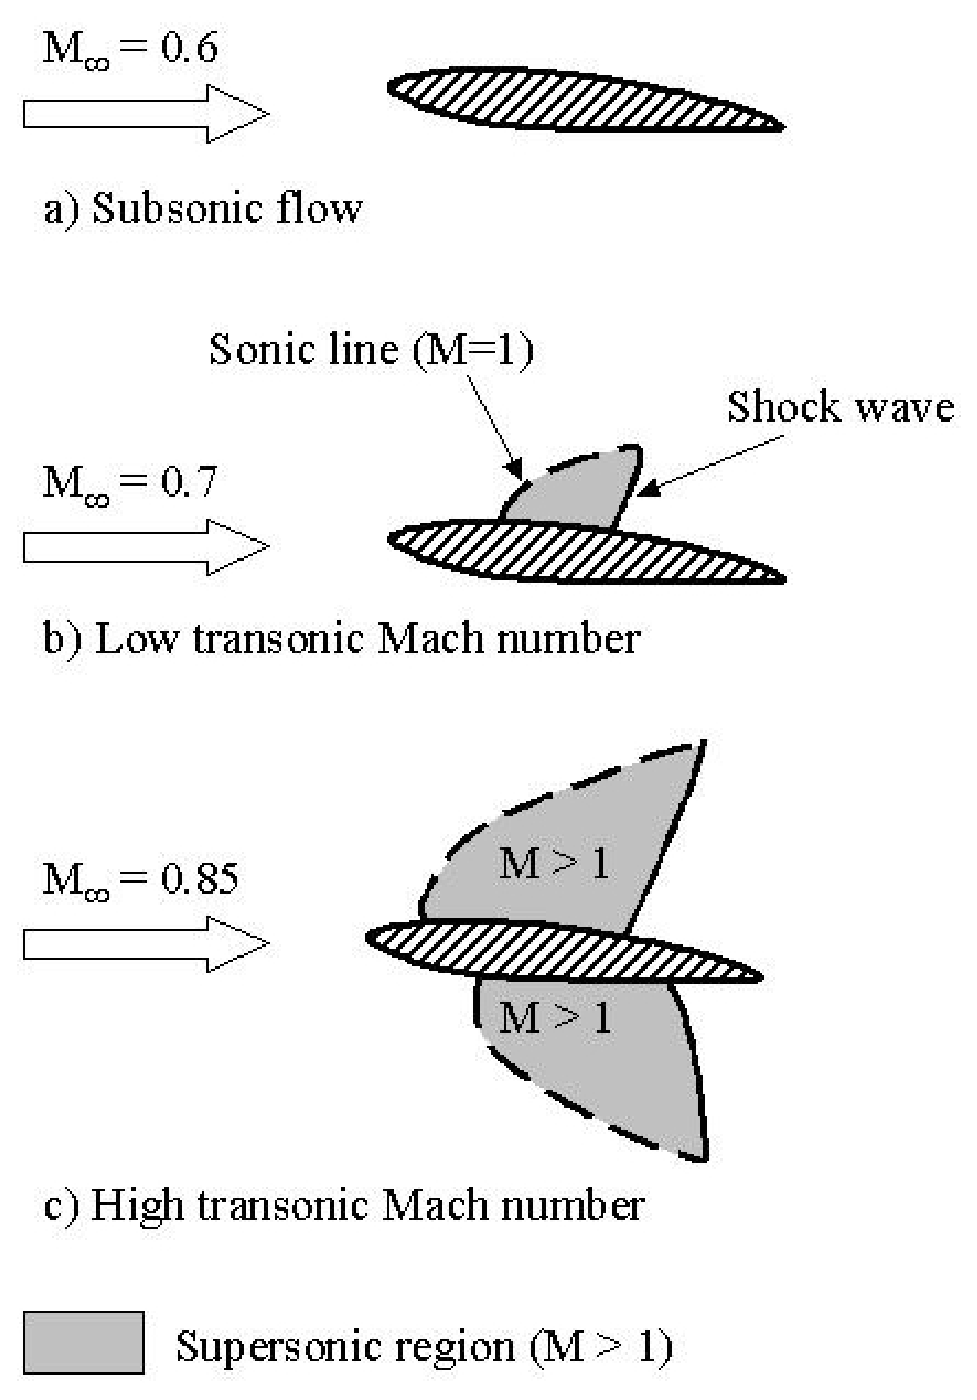
\includegraphics[height=6in]{aflow}
%     \else
%       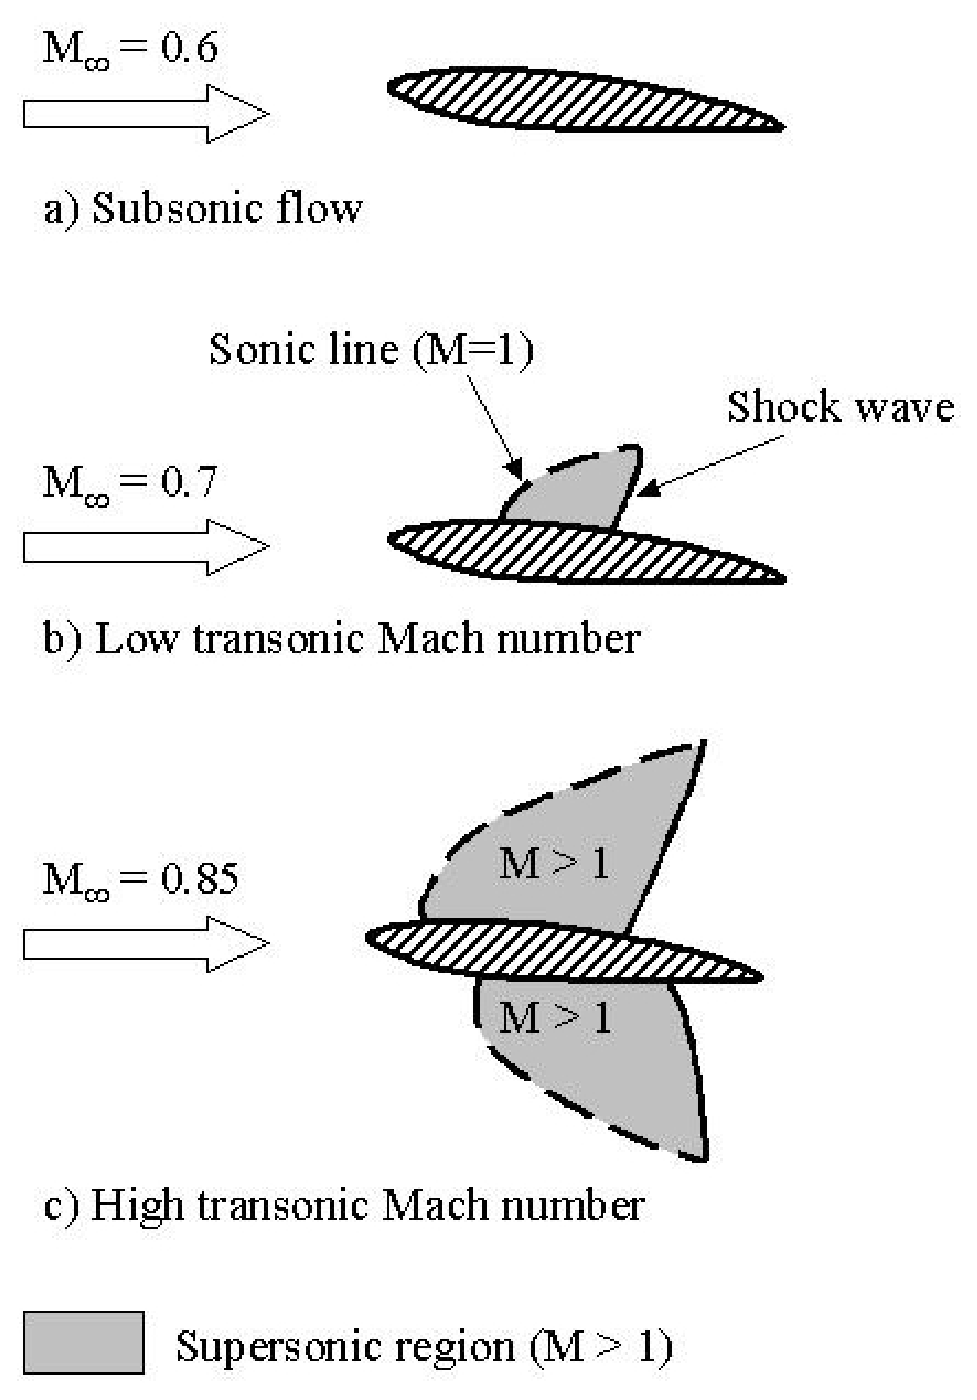
\includegraphics[bb = 92 86 545 742, height=6in]{aflow}
%     \fi
%     \caption{Airfoil Picture}
%     \label{FigAir}
%   \end{center}
% \end{figure}

% above code has been macro-fied in Classes/MacroFile.tex file
%\InsertFig{\IncludeGraphicsH{aflow}{6in}{92 86 545 742}}{Airfoil Picture}{FigAir}

% So as we have now labelled it we can reference it, like so (\ref{FigAir}) and it
% is on Page \pageref{FigAir}. And as we can see, it is a very nice picture and we
% can talk about it all we want and when we are tired we can move on to the next
% chapter ...

% I would also like to add an extra bookmark in acroread like so ...
% \ifpdf
%   \pdfbookmark[2]{bookmark text is here}{And this is what I want bookmarked}
% \fi
% ------------------------------------------------------------------------


%%% Local Variables: 
%%% mode: latex
%%% TeX-master: "../thesis"
%%% End: 

\chapter{Methodology}
\ifpdf
    \graphicspath{{Chapter2/Chapter2Figs/PNG/}{Chapter2/Chapter2Figs/PDF/}{Chapter2/Chapter2Figs/}}
\else
    \graphicspath{{Chapter2/Chapter2Figs/EPS/}{Chapter2/Chapter2Figs/}}
\fi

\section{Baseline Method}

\begin{figure}[!htbp]
  \begin{center}
    \leavevmode
    \ifpdf
      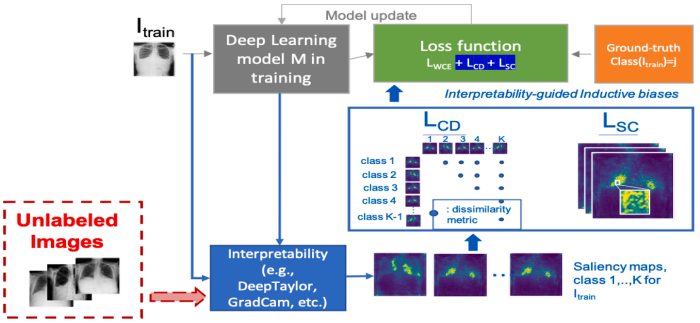
\includegraphics[scale=0.75]
      {Chapter2/Chapter2Figs/sibnet_arch.png}    
    \fi
    \caption{Sibnet Architecture}
    \label{sibnet_arch}
  \end{center}
\end{figure}

We now detail the idea proposed by \cite{MAHAPATRA2022102551} in the paper titled "Interpretability Guided Inductive Bias for Deep Learning Based Medical Image". This is the paper we started out with to reproduce the results of.

The paper takes inspiration from the observation that when a radiologist is performing diagnosis on medical images, they look for disease-specific image patterns or characteristics. We attempt to help the model imitate the same by integrating a novel inductive bias in the loss term of the model along with cross entropy loss such that the learned features yield more class distinctive and spatially coherent saliency maps which makes it easier for the radiologist to diagnose. The bias term we define acts directly on the loss function of the model being trained, it is modular and easy to implement, and can be used in combination with any other loss functions, as well as on existing classification model architectures without any modifications

Figure \ref{sibnet_arch} shows the main pipeline of the approach. A model is trained with a combination of standard classification loss terms and the proposed interpretability-guided inductive bias loss terms. The learned features obtained from the model generate more class distinctive and spatially coherent saliency maps. This makes the learned features of a class as unique as possible from features of other classes and that improves the model performance. Moreover, it enforces an enhanced spatial attention to the class label describing the targeted disease. This helps the radiologist a lot in understanding which regions of an x-ray image describe a particular disease and makes the diagnosis easier. Any deep learning model can be used with our proposed loss term. The paper uses DenseNet121 as it has performed well on medical images classification and it has skip connections which eliminates the problem of vanishing gradients. It is very crucial that we don’t face vanishing gradients problem for this specific task as we use gradients to generate saliency maps.

A saliency map \textbf{$S_{\{I,c\}} \in R^d$}
identifies important regions of an image I which are to
be classified as label c for a given training image I and model M. The proposed
inductive bias aggravates the distinctiveness between saliency maps \textbf{$S_{\{I,c=i\}}$} and \textbf{$S_{\{I,c=j\}} (j \ne i) (\forall i, j \in \{1, ...., K\})$} for different classes of an image I and improves spatial coherence to effectively identify the features of an image used by the model
to perform classification. Two loss terms were proposed to handle separate aspects of multi-class classification.

\subsection{Class distinctiveness Loss}

Given training image $I$ and model $M$, we generate a set of saliency maps $\left\{S_{I, c}\right\}_{c=1}^{K}$ which encodes the explanation for each class $c$. Then, we compute the corresponding latent representations of the saliency maps $\left\{Z_{S_{I, c}}\right\}_{c=1}^{K}$ from the last convolutional layer of the model. The latent representation vectors $Z$ encode the current understanding of the model $M$ to the generated saliency maps.

In order to induce distinctiveness of saliency maps of an image among different classes, we calculate the loss term $\left(L_{C D}\right)$, as follows:

\begin{center}
{ $L_{C D}=\frac{2}{K(K-1)} \sum_{c_{1}=1}^{K-1} \sum_{c_{2}=c_{1}+1}^{K}$ cosine\_similarity $\left(Z_{S_{l, c_{1}}}, Z_{S_{I, c_{2}}}\right)$}
\end{center}


In the above equation, cosine\_similarity(.) is the cosine similarity metric that computer dissimilarity of 2 vectors where 1 denotes minimum dissimilarity and  0 denotes maximum dissimilarity. We take the average of cosine similarity of all possible pairs of latent representations for an image. The basic intuition make the latent representations $Z$ as dissimilar as possible from each other. Any other similarity metric can be used instead of cosine similarity. As the model training minimizes the loss function, the model eventually learns to minimize the similarity among different latent representations for an image. 

\subsection{Spatial coherence loss}

The objective of the spatial coherence loss term is to regularize the spatial distribution of saliency maps. This function aims to reduce the dispersion of features of saliency maps by making the features as cohesive as possible as that would be closer to the regions annotates by experts and makes it easier for doctors to identify the region of interests with more certainty and perform diagnosis. We propose a spatial coherence loss term $\left(L_{S C}\right.$ ), as follows:

\begin{center}
{$L_{S C}=\sum_{p} \sum_{n_{p} \in \mathscr{T}(p)}\left\|x_{p}-x_{n_{p}}\right\|^{2}$}
\end{center}

In the above equation, $x_{p}$ is the pixel intensity in saliency map $S_{I, c}$ and $x_{n_{p}}$ is the set of pixels in the $9 \times 9$ neighborhood $\mathscr{N}(p)$ belonging to the same cluster as p. 
A small neighbourhood may not provide adequate information about the local neighbourhood whereas the computational complexity is too much for large neighborhood. $9 \times 9$ neighborhood was able to achieve good accuracy with decent computational complexity. Clusters on each saliency map are identified by performing connected component analysis. This loss term penalises the difference in intensity between pixels belonging to same cluster located in a neighborhood and thus ensures that the pixels of same cluster in a neighborhood have similar intensity values making them more spatially coherent.

The total loss is defined as: 
$L_{\text {Total }}=L_{W C E}+\lambda_{1} L_{C D}+\lambda_{2} L_{S C}$ where
$\lambda_{1}$ and $\lambda_{2}$ are the parameters that determine the contribution of class distinctiveness and spatial coherence loss respectively to the loss function.

\section{GradCAM}
GradCAM is a technique to generate saliency maps mainly for Convolutional Neural Networks. There can be various methods to obtain saliency maps as explained in Chapter \ref{chap:litreview}. In our project we have mainly used the Gradient Weighted Class Activation Mapping (GradCAM) \cite{selvaraju2017grad}.
It uses the gradients flowing to the final convolutional layer over any target to produce a coarse localization maps highlighting the important regions used to predict the target.\\
\begin{figure}[!htbp]
  \begin{center}
    \leavevmode
    \ifpdf
      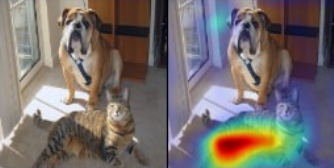
\includegraphics[scale=1]
      {Chapter2/Chapter2Figs/gradcam.png}    
    \fi
    \caption{GradCAM Saliency Map Visualization for "tiger cat" category for VGG16 network, \cite{selvaraju2017grad}}
    \label{gradcam_eg}
  \end{center}
\end{figure}

The gradients of the target class's score with respect to the final convolutional layer of the CNN are calculated by backpropagating the gradients from the output layer to the final convolutional layer, considering only the target class's score and ignoring the other classes. These gradients represent the importance of each channel in the final CNN layer. To quantify the importance of each channel, he activation maps are then averaged over the whole channel. These weights are then finally used to weigh the activation maps across different channels and combine them. ReLu Activation is applied at the end to obtain only non-negative contributions.

Finally the final feature map obtained may be in size smaller than input image. To overcome this the feature map is upsampled using techniques like \textbf{Bilinear Interpolation}.


\section{Modified Pipeline}

\begin{figure}[!htbp]
  \begin{center}
    \leavevmode
    \ifpdf
      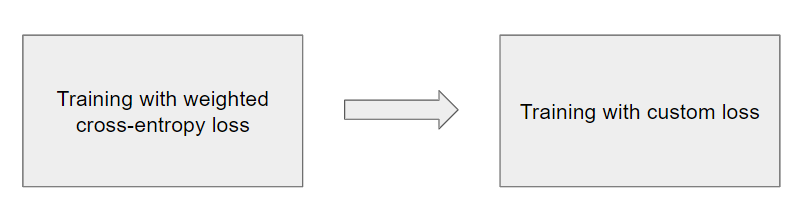
\includegraphics[scale=0.85]
      {Chapter2/Chapter2Figs/modified_pipeline.png}    
    \fi
    \caption{Modified Pipeline}
    \label{mod_pipe}
  \end{center}
\end{figure}

In the given baseline method, the model is trained on the proposed loss functions from scratch. This means that the model starts learning from the pre trained weights as we use pre trained weights of the given architecture. Since both Class Distinctiveness Loss and Spatial Coherence Loss rely on saliency maps, it is important that the saliency maps generated are of adequate quality which means that the saliency maps contain relevant information to help the model better. However, the saliency maps generated in the beginning will not have any information about the location of the object(disease in this case) as the models were pre trained on natural domain images and have no information regarding medical images. Therefore, the initially generated saliency maps may mislead the model and the model may not achieve the desired convergence.

In order to overcome this issue, we propose a modified pipeline of training the model. Figure \ref{mod_pipe} shows the pipeline we have proposed. First we train our model using weighted cross entropy loss only. Once this is done, the model would have learnt the features of the diseases well which leads to better quality of saliency maps with relevant information about the location of the disease learnt by the model. Then, we train our model using the custom loss function. Now, the proposed loss functions will leverage the good quality information provided by the saliency maps to achieve even better performance and saliency maps. Once the training of modified pipeline is done, we can expect to achieve more class distinctive and spatially coherent saliency maps and increase in performance of the model than when compared to training the model on just the custom loss function.  

\section{Loss Functions to address Class Imbalance}

There were few issues with the loss functions proposed in the baseline method. The first issue was that the model training was at least 4 times slower with the custom loss functions than with just cross entropy loss. We attribute this poor performance to the computational complexity of calculating saliency maps. We performed a small experiment where we just fed random data instead of generating saliency maps and then feeding them. We observed that there was no difference in training time between custom loss and cross entropy loss when saliency maps are not generated. Thus, we concluded that generating saliency maps was computationally expensive and there is a need to trade-off between model training time and model performance.

The second issue was that the model performance didn't improve with the custom loss function. The model performance was actually worse with the custom loss functions. Although we were able to close the gap with our modified pipeline, the two proposed loss functions essentially didn't improve the model performance over the standard cross entropy loss function. We concluded that we couldn't improve the performance of the model with the help of performance. We couldn't compare the quality of saliency maps generated by models trained with different loss functions as we neither have the ground truth label of the disease nor the domain expertise to analyse the saliency maps. 

Therefore, we decided to solve a slightly different problem that arises in multi-label medical classification models rather than interpretability. We investigated the class imbalance problem. We found that when the model is trained with weighted cross entropy, there was a huge gap in performance between different classes. For instance, we obtained an AUC of 0.867 for Atelectasis, whereas we obtained an AUC of just 0.691 for Edema. Therefore, we incorporated two new loss functions to address class imbalance problem named Focal Loss introduced by \cite{lin2017focal} and Deep AUC Maximization proposed by \cite{yuan2021large}.

\subsection{Focal Loss}

Focal Loss was first introduced to mainly solve the class imbalance problem in the context of object detection. They discovered that the extreme foreground-background class imbalance encountered
during training of dense detectors is the central cause. They address this class imbalance by reshaping the
standard cross entropy loss such that it down-weights the
loss assigned to well-classified examples. Focal Loss focuses on ensuring predictions improve over hard examples rather than becoming overconfident with easy cases.

It is a dynamically scaled cross entropy loss, where the scaling factor decays to zero as confidence in the correct class increases. Intuitively, this scaling factor can automatically down-weight the contribution of easy examples during training and rapidly focus the model on hard examples. The Focal Loss adds a factor $(1-p_t)^\gamma$ to the standard cross entropy criterion. Setting $\gamma>0$
 reduces the relative loss for well-classified examples $(p_t>0.5)$, putting more focus on hard, misclassified examples. There is a tunable focusing parameter $\gamma\geq0$. 

 Although it was introduced initially to solve class imbalance problem in object detection of objects from natural domain, focal loss has also been used in medical image classification problems down the line \cite{lotfy2019investigation} \cite{tran2019improving} and showed good performance in such settings. This gave us the confidence to go ahead with focal loss. We essentially replace cross entropy loss with focal loss. Focal loss is formally defined as:

 \begin{center}
{ $L_{focal}=-\sum_{i=1}^{i=n}(1-p_i)^{\gamma}log(p_i)$}
\end{center}


\subsection{Deep AUC Maximization}
Deep AUC Maximization is a paradigm to learn deep learning networks with the objective of maximizing the area under the ROC curve, the AUC. Unlike other loss functions mentioned above, DAM directly aims to optimize the AUC rather than minimizing the loss like cross entropy loss.

According to \cite{yuan2021large}, as in medical classification tasks AUC is already the default metric for performance measure during training or evaluating, directly maximizing it helps to increase performance fastest.
Secondly, it is helpful to the medical imaging setting due to the class imbalance nature of datasets, owing to anomalies appearing less often. This is because AUC is more suitable to handle imbalanced data distribution, since maximizing AUC aims to rank score of any positive data higher than any negative data.

AUC according to Wilcoxon-Mann-Whitney statistic is defined as:
\begin{center}
{\textbf{$AUC(w) = Pr(h_w(x) \geq h_w(x')|y = 1, y' = -1)$}}
\end{center}
Above simplifies to, 
\begin{center}
{\textbf{$AUC(w) = Pr(I(h_w(x) - h_w(x'))\geq 0|y = 1, y' = -1)$}}
\end{center}
In general, the Identity function can be replaced by some surrogate loss function, \emph{l}, in our experiments we have used the surrogate loss function, proposed in the paper \cite{yuan2021large} provided via the \textbf{libauc} library:
\begin{center}
{\textbf{$AUC(w) = Pr(\emph{l}(h_w(x) - h_w(x'))\geq 0|y = 1, y' = -1)$}}
\end{center}
\section{MIMO Networks}

The current setup of multi label classification takes in one image as input and outputs probability values for each class. This can be called a single input multiple output setup. The best performance in classifying the Chexpert dataset has been obtained by ensembles of neural networks. Ensembles use more than one neural network and combine their predictions to obtain more accurate and robust predictions, the idea being different models have different strengths and weaknesses.

But using ensembles adds a lot to the computational requirements. \cite{havasi2021training} propose the idea of Multiple Input Multiple Output (MIMO) Networks which help reduce the number of forward passes and hence compute requirements. They utilize a single model’s capacity to train multiple subnetworks that independently learn the task at hand.

\begin{figure}[!htbp]
  \begin{center}
    \leavevmode
    \ifpdf
      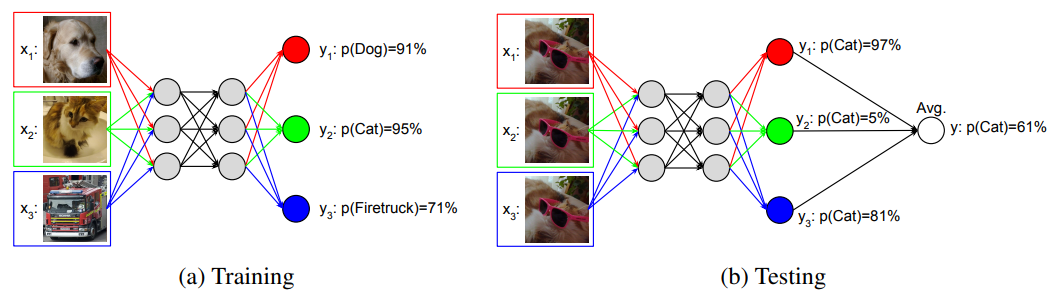
\includegraphics[scale=0.5]
      {Chapter2/Chapter2Figs/mimo.png}    
    \fi
    \caption{Figure Showing the training and testing procedures in MIMO networks}
    \label{mimo}
  \end{center}
\end{figure}

Fig.\ref{mimo} shows the training and testing pipelines for a toy neural network. Number of outputs in a MIMO network need to be equal to the total number of classes like in regular single input multiple output classification networks. But, it needs multiple images as inputs. During training the input images can be different, while during testing, all the input images have to be same.

Results in \cite{havasi2021training} show robustness of the model was improved by ensembling the predictions made by the subnetworks without increasing compute.Particularly, significant improvement in negative log-likelihood, accuracy, and calibration error was observed.

\section{Model Calibration}

Model Calibration is the method of adjusting the predictions made by a trained model to improve their reliability or align them with the desired outcome probabilities. This becomes crucial when using machine learning models in domains where well-calibrated probabilities are essential for informed actions or risk assessments. We don't just want the model to give outputs but also make sure that the model predicts with right amount of confidence. Let's say we have a binary classifier and it predicts an instance with the value 0.6. Although we may interpret it as belonging to class 1, it is important to understand that the model predicted it as class 1 with only 60\% confidence. In a real life medical setting, it is important that the model predictions are neither underconfident nor overconfident. 

\begin{figure}[!htbp]
  \begin{center}
    \leavevmode
    \ifpdf
      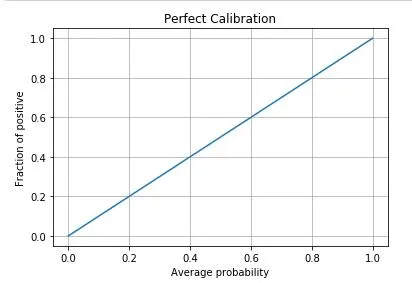
\includegraphics[scale=0.7]
      {Chapter2/Chapter2Figs/per_cal.png}    
    \fi
    \caption{The plot of a perfectly calibrated model}
    \label{per_cal}
  \end{center}
\end{figure}

In order to align the model probabilities with ground truth distribution and predict with appropriate confidence, we calibrate the model outputs. Various methods have been proposed over the years to calibrate the model probabilities like Histogram Binning (\cite{zadrozny2001obtaining}), Isotonic regression (\cite{zadrozny2002transforming}), Bayesian Binning (\cite{naeini2015obtaining}), Platt Scaling (\cite{platt1999probabilistic}) and Temperature scaling (\cite{guo2017calibration}. However, we decided to go ahead with temperature scaling for calibrating the model probabilities due to the promise it showed in calibrating model probabilities of various CNN models such as DenseNet and ResNet when trained on popular datasets like ImageNet and CIFAR-100.

\subsection{Temperature Scaling}

Temperature Scaling is a post-processing technique that was proposed by \cite{guo2017calibration} to improve upon the calibration error by dividing the logits by a learned scalar parameter called Temperature. It is an extension of Platt scaling and uses a single scalar parameter T > 0 for all classes where T is the temperature. Temperature is learned by minimizing the negative log likelihood between model logits divided by temperature and true values. The new softmax function which provides the calibrated probabilities is given as:

\begin{center}
{ $softmax=\frac{e^{z/T}}{\sum_ie^{z_i/T}}$}
\end{center}

When $T>1$, the softmax values is softened, in other words the output entropy is raised. As T → $\infty$, the probability $p_i$ approaches 1/N, which represents maximum uncertainty. With T = 1, we recover the original
probability $p_i$. As T → 0, the probability collapses to a
point mass (i.e. $p_i$ = 1). One more thing to note is that since the parameter T does not change the maximum of the softmax function, the class
prediction does not change on applying Temperature Scaling.

% ------------------------------------------------------------------------

%%% Local Variables: 
%%% mode: latex
%%% TeX-master: "../thesis"
%%% End: 

\chapter{Experiments}
\ifpdf
    \graphicspath{{Chapter3/Chapter3Figs/PNG/}{Chapter3/Chapter3Figs/PDF/}{Chapter3/Chapter3Figs/}}
\else
    \graphicspath{{Chapter3/Chapter3Figs/EPS/}{Chapter3/Chapter3Figs/}}
\fi

\section{CheXpert Dataset}

The CheXpert (\cite{irvin2019chexpert}) dataset contains 224,316 chest radiographs of 65,240 patients with both frontal and lateral views available. This dataset was created to perform automated chest x-ray interpretation, featuring uncertainty labels and radiologist-labeled reference standard evaluation sets. This is a multi-label dataset containing 14 chest disease labels that can be detected using x-ray images. A multi-label dataset is a dataset which has more than one output class with label 1 for a given input. In this context, a patient can have more than one disease which is reflected in the dataset as well. Some images are of 320 x 320 and some are of 390 x 320. This dataset has both frontal and lateral views. However, we have reduced the image size in our training setup to 224 x 224 in order to match the input shape of the neural network model.

The performance of the model trained on CheXpert is evaluated using the provided validation set which has 200 images. However, the validation set has only 5 disease labels. So, we have considered only 5 corresponding disease labels for training to maintain consistency. The diseases considered are  Atelectasis, Cardiomegaly, Consolidation, Edema and Pleural Effusion. Every disease has 3 labels: either 0(negative), 1(positive), -1(uncertain). There are various ways to handle the uncertain labels as shown in \cite{irvin2019chexpert}. We have assigned label 1 to Cardiomegaly and Edema and label 0 to the rest 3 diseases as it has been empirically found that this way of modifying uncertain labels has shown the most appropriate results. 

\section{Metrics}

\subsection{AUC}

\begin{figure}[!htbp]
  \begin{center}
    \leavevmode
    \ifpdf
      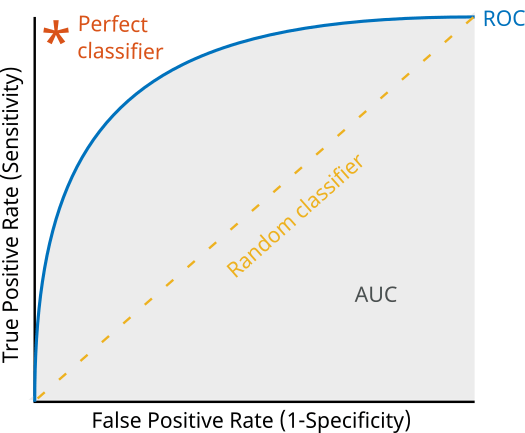
\includegraphics[scale=0.4]
      {Chapter3/Chapter3Figs/AUC.png}    
    \fi
    \caption{AUC (Area under the ROC Curve)}
    \label{auc}
  \end{center}
\end{figure}

AUC stands for Area under the ROC Curve. An ROC curve (receiver operating characteristic curve) is a graph showing the performance of a classification model at all classification thresholds. This curve plots two parameters: True Positive Rate (TPR) and False Positive Rate (FPR). True Positive Rate is the probability that an actual positive sample is classified as positive. False Positive Rate is the probability that an actual negative sample is misclassified as positive. An ROC curve plots TPR vs. FPR at different classification thresholds. AUC measures the entire two-dimensional area underneath the entire ROC curve from (0,0) to (1,1). Higher the AUC value, better the model performance. 



\subsection{Expected Calibration Error}

Expected Calibration Error quantifies how well a given model is calibrated i.e how well the predicted output probabilities of the model matches the actual probabilities of the ground truth distribution. Expected Calibration Error was introduced by \cite{naeini2015obtaining}. In computing ECE, the predictions are sorted and partitioned into N fixed number of bins (N = 15 in our experiments). The predicted value of
each test instance falls into one of the bins. The ECE calculates Expected Calibration Error over the bins. The formula of Expected Calibration Error is given as:

\begin{center}
{ $ECE=\sum_{i=1}^Nb_i||p_i-c_i||$}
\end{center}


\section{Evaluation of baseline methods and modified pipeline}

\begin{table}[htbp]
\centering
\begin{tabular}{|p{1.5cm}|p{2.25cm}|p{2.25cm}|p{2.25cm}|p{1.5cm}|p{2.25cm}|p{1.25cm}|}
  \hline
  Loss & Atelectasis & Cardiomegaly & Consolidation & Edema & Pleural Effusion & Mean\\
  \hline
  Cross Entropy  &  0.769 &
0.764 &
0.751 &
0.675 &
0.822 &
0.756
\\
  \hline  
  Custom &  0.722 &
0.807 &
0.743 &
0.645 &
0.806 &
0.745

\\
  \hline
  Modified Pipeline &  0.752 &
0.810 &
0.716 &
0.646 &
0.822 &
0.749

\\
  \hline
\end{tabular}
\caption{\label{baseline_results}Table Showing Performance Comparison (Validation AUC values) on model trained on 15 epochs of Cross Entropy Loss, Class Distinctiveness Paired with Cross Entropy and the Double Stage Pipeline with Class Distinctiveness and Cross Entropy Losses}
\end{table}

We perform an ablation study on the baseline loss functions introduced in \cite{MAHAPATRA2022102551}. 
We trained and validated the DenseNet121 model only with the crossentropy loss and the crossentropy loss coupled with the class distinctiveness loss. We don't present here the results when the spatial coherence loss is considered, as the model training takes too much time when the spatial coherence loss is incorporated and it doesn't seem to converge within reasonable time limits. 

For the cross entropy loss with the class distinctiveness loss, we try two approaches. First, training the model from random initial weights with both the loss terms. Second, training the model first only on the weighted cross entropy followed by further training the model on the modified loss term with class distinctiveness loss. The results of all the three approaches when trained and validated on 15 epochs is as shown in Table \ref{baseline_results}.

The two stage training schedule is expected to perform better and achieve faster convergence because of the concern of the model diverging if classdistinctiveness is used at the beginning with \textbf{bad  saliency maps}, i.e. model not good enough to get relevant saliency maps.
The best AUC from Table \ref{baseline_results} seem to appear from the Cross Entropy loss only, followed by the custom loss using the double stage modified pipeline and followed by the standard custom loss, single stage pipeline.

\begin{figure}[!htbp]
  \begin{center}
    \leavevmode
    \ifpdf
      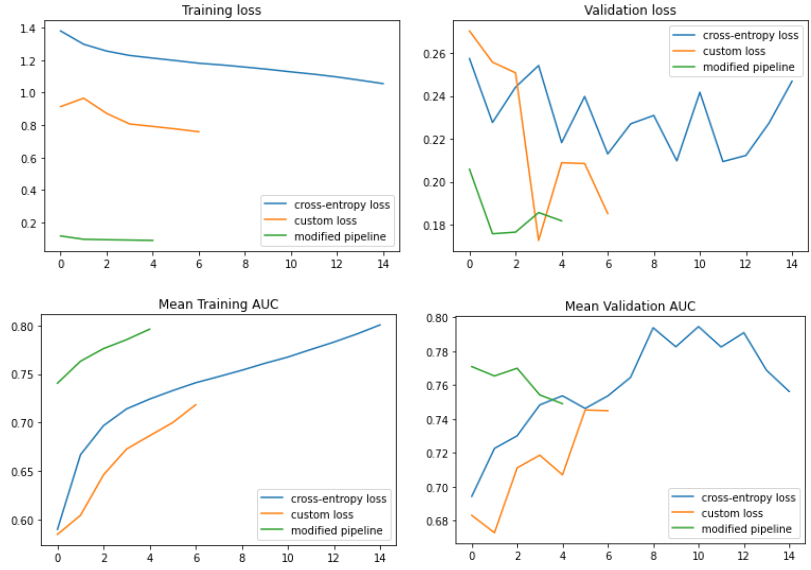
\includegraphics[scale=0.5]
      {Chapter3/Chapter3Figs/baseline_gs.png}    
    \fi
    \caption{Plots showing the training and validation loss and auc vary with number of epochs}
    \label{baseline_res}
  \end{center}
\end{figure}
When experimenting with custom loss using class distinctiveness loss, we do grid search for the hyperparameter $\lambda_1$, to get optimal value almost 1.4 as suggested in the paper.

\section{Debugging Class Distinctiveness Loss}
Class distinctiveness loss, does one thing well, it makes sure the saliency maps corresponding to different maps look reasonably different. But it doesn't necessarily give maps close to the reality. Not knowing the ground truth makes for the model hard to converge.
 Other hyperparameters like $\lambda_1$, learning rate and drop out rate were changed to obtain optimal ones. Still finally the custom loss usually achieved performance atmost as good as the cross-entropy loss.
 \begin{figure}
  \centering
  \begin{minipage}[b]{0.45\textwidth}
    \centering
    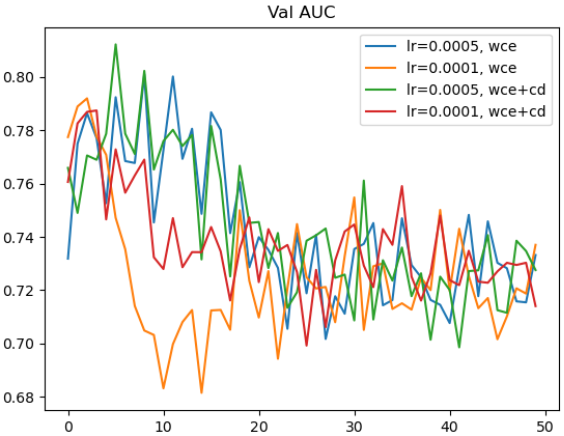
\includegraphics[width=\textwidth]{Chapter3/Chapter3Figs/lr.png}
    \caption{Graph showing val AUC vs number of epochs for model trained for 50 epochs for different learning rates}
    \label{fig:lr}
  \end{minipage}
  \hfill
  \begin{minipage}[b]{0.45\textwidth}
    \centering
    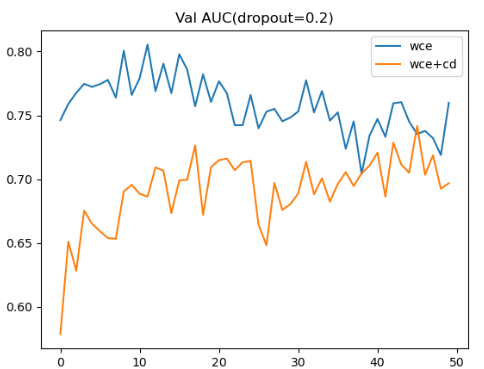
\includegraphics[width=\textwidth]{Chapter3/Chapter3Figs/drop.png}
    \caption{Graph showing val AUC vs number of epochs for model trained for 50 epochs for different dropout rates}
    \label{fig:drop}
  \end{minipage}
\end{figure}
\section{Experiments with Different Architectures}
We also experimented with 3 different backbone networks with other factors same. Namely we used the Densenet-121, Resnet-101 and VGG-19 as our model backbones
All the three backbone based methods, after 15 epochs obtained AUCs of over 0.8. The saliency maps corresponding to the three methods, are plotted in \ref{sal_diff_loss}.
\begin{figure}[!htbp]
  \begin{center}
    \leavevmode
    \ifpdf
      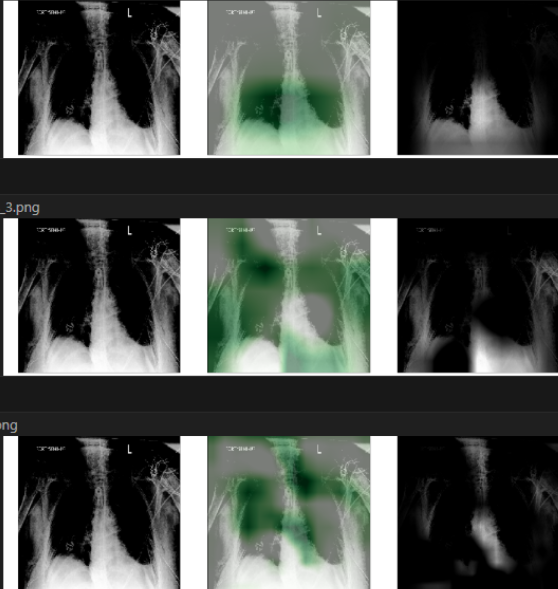
\includegraphics[scale=0.6]
      {Chapter3/Chapter3Figs/sal_arch}    
    \fi
    \caption{Saliency Maps for models trained with different backbone networks, top row for Cross Entropy Loss, middle row for Resnet101, and third VGG-19}
    \label{sal_diff_loss}
  \end{center}
\end{figure}
\section{Experiments with newly introduced loss functions}

\begin{table}[htbp]
\centering
\begin{tabular}{|p{1.8cm}|p{1.9cm}|p{2.4cm}|p{2.4cm}|p{1.3cm}|p{1.5cm}|p{1.1cm}|}
  \hline
   Loss Function & Atelectasis & Cardiomegaly & Consolidation & Edema & Pleural Effusion & Mean \\
  \hline
  Cross Entropy Loss &  0.8350 & 0.9032 & 0.9120 & 0.8489 & 0.9217 & 0.8841 \\
  \hline  
  Focal Loss & 0.8568 & 0.9077 & 0.9016 & 0.8447 & 0.9230 & 0.8867 \\
  \hline
  DeepAUC Loss & 0.7368 & 0.8263 & 0.9160 & 0.8269 & 0.8393 & 0.8291 \\
  \hline
\end{tabular}
\caption{\label{diffloss} Performance comparison (Validation AUC) across different loss functions}
\end{table}

\begin{figure}[!htbp]
  \begin{center}
    \leavevmode
    \ifpdf
      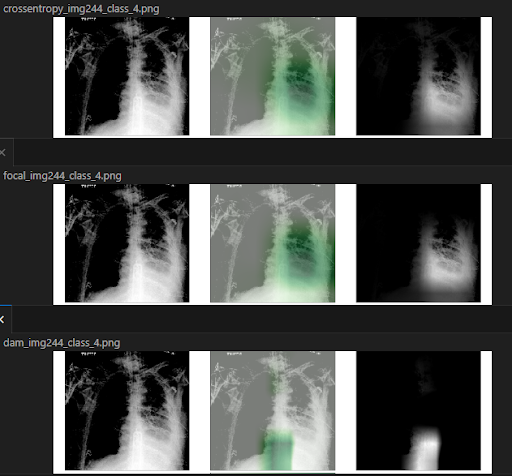
\includegraphics[scale=0.6]
      {Chapter3/Chapter3Figs/sal_diff_loss.png}    
    \fi
    \caption{Saliency Maps for all 3 models trained with different loss functions over an image.}
    \label{sal_diff_loss}
  \end{center}
\end{figure}

As we introduced Focal Loss and Deep AUC Maximization, we trained our DenseNet121 model on CheXpert dataset to analyse its performance under different loss functions. We used Adam Optimizer with a learning rate of 1e-4 and weight decay of 1e-5. We fixed the batch size of training data as 64 and trained our model for 5 epochs across all loss functions. One more interesting thing to note here is that we were able to improve the performance of model trained with Cross Entropy Loss from just 0.80 AUC to 0.88 AUC by finding and utilizing better hyperparameters. 

The results obtained are displayed in the table \ref{diffloss}. We can observe that Focal Loss has performed marginally better than Cross Entropy Loss. DeepAUC Loss, however, is not able to match the performance of other two loss functions, despite its objective being maximizing the very metric that is used to evaluate the model. 

In addition, we have also obtained the saliency maps of the models trained with these loss functions over a sample image as shown in figure \ref{sal_diff_loss}. The top, middle and bottom rows denote Cross Entropy Loss, Focal Loss and Deep AUC Loss. The left column denotes the input image and the next two columns display the obtained saliency maps denoting the regions learnt by the model pertaining to certain class. Here, we have obtained the region pertaining to class 4 for different models. We can observe that the saliency maps obtained for Cross Entropy Loss and Focal Loss are almost identical. We can probably attribute that to the fact that the mathematical form of Cross Entropy Loss and Focal Loss are almost identical, thus they learnt in an almost identical manner. It could also be possible that the both models have learnt well for the particular class and thus generated identical saliency maps. The saliency map obtained for DeepAUC Loss looks different when compared to the other two loss functions. As displayed in table \ref{diffloss}, DeepAUC Loss is less accurate than the other two loss functions, so probably the saliency map generated DeepAUC Loss is not accurate. However, we don't have any way to verify our findings and hypotheses due to lack of domain knowledge i.e the ability to diagnose diseases using chest x-rays in this context. Therefore, we can't perform qualitative analysis of saliency maps with certainty. 

\section{Calibration of the trained models}

\begin{table}[htbp]
\centering
\begin{tabular}{|p{1.8cm}|p{3.2cm}|p{3.2cm}|}
  \hline
   Loss Function & Mean ECE before calibration & Mean ECE after calibration \\
  \hline
  Cross Entropy Loss & 0.1147 & 0.0996 \\
  \hline  
  Focal Loss & 0.1763 & 0.1091 \\
  \hline
  DeepAUC Loss & 0.2348 & 0.0992 \\
  \hline
\end{tabular}
\caption{\label{ece} Mean ECE before and after calibrating the model using Temperature Scaling}
\end{table}

We calibrated the models trained under 3 different loss functions using Temperature Scaling. We have compared the calibration errors obtained before and after calibration for all 3 loss function in table \ref{ece}. We can observe that in all 3 cases, the mean ECE has reduced after calibration. We can also observe that the model trained with Cross Entropy Loss is the most calibrated model which means that the predictions of the model are closer to the ground truth distribtion and thus more reliable, even though the model trained with Focal Loss obtained marginally better AUC. Therefore, the model trained with Cross Entropy Loss is the most reliable model and the model performance is almost as good as the best one. After calibration though, all 3 models have similar mean ECE values. So after calibration, all 3 models are equally reliable. The drop in ECE value after calibration, especially in the case of DeepAUC Loss which is around 0.1356, shows that calibration is a very important step after the model training is completed to improve the reliability of the model which is very important in critical medical applications. 

% ------------------------------------------------------------------------


%%% Local Variables: 
%%% mode: latex
%%% TeX-master: "../thesis"
%%% End: 

\include{Chapter4/chapter4}
\def\baselinestretch{1}
\chapter{Conclusion}
\ifpdf
    \graphicspath{{Conclusions/ConclusionsFigs/PNG/}{Conclusions/ConclusionsFigs/PDF/}{Conclusions/ConclusionsFigs/}}
\else
    \graphicspath{{Conclusions/ConclusionsFigs/EPS/}{Conclusions/ConclusionsFigs/}}
\fi

\def\baselinestretch{1.66}

We have investigated the role of interpretability and calibration in medical image classification tasks. We were unable to show any improvement with the help of loss functions which are Class Distinctiveness Loss and Spatial Coherence Loss. We improved the performance of custom loss function by using our proposed modified pipeline. However, the performance of the modified pipeline was still worse than the Weighted Cross Entropy model. We attempted to fix this by changing various hyperparameters like learning rate, dropout rate and $\lambda1$ value. Despite our efforts, we were not able to show any significant improvement. Moreover, we were not able to verify the quality of saliency maps generated by different methods as we don't have expertise in medical domain. We also experimented with different architectures apart from DenseNet121 such as ResNet101 and VGG19. We also explored the possibility of using Multi Input Multi Output (MIMO) Network in our training setup.

We pivoted in a different direction by studying the class imbalance problem. The 5 classes we chose for training and evaluation from the CheXpert didn't have a balanced representation of each class. This imbalance reflected in the model performance too as the AUC of each class varied with each other. We incorporated two new loss functions which are Focal Loss and DeepAUC Loss. We analysed the model performance under 3 different loss functions and found Focal Loss to perform marginally better than Cross Entropy Loss. DeepAUC Loss was not able to match performance of other two loss functions. Meanwhile, we were able to improve the mean AUC of Cross Entropy model from 0.80, which we obtained in our earlier experiments, to 0.88 which we attribute to using better set of hyperparameters. We also wanted to make sure that our trained models are reliable enough for deployment in real life applications which is very important in the context of medical domain. We investigated how calibrated the model probabilities are and further calibrated them using Temperature Scaling. We observed that the Cross Entropy model was the most calibrated, however all 3 models were calibrated to similar degree as the Expected Calibration Errors decreased for all 3 models after applying Temperature Scaling. Most of the medical classification models mainly focus on the accuracy only without focusing on the model calibration. We argue that it is very important to calibrate the models and the same reflected in our experiments as well. We have analysed the effects of using saliency maps to improve accuracy and interpretability, investigated the use of different loss functions to address class imbalance problem and proved the importance of model calibration.

%%% ----------------------------------------------------------------------

% ------------------------------------------------------------------------

%%% Local Variables: 
%%% mode: latex
%%% TeX-master: "../thesis"
%%% End: 


\backmatter % book mode only
\appendix

\bibliographystyle{plainnat}
%\bibliographystyle{Classes/IITRPRbiblio}
\renewcommand{\bibname}{References} % changes default name Bibliography to References
\bibliography{References/references} % References file

\end{document}
